\documentclass[a4paper]{memoir}

\usepackage[utf8]{inputenc} \usepackage{geometry}
\usepackage{amsmath, amsfonts, amssymb, amsthm, mathtools}
\usepackage{graphicx}
\usepackage{parskip}
\usepackage{fancyhdr}
\usepackage{lastpage}
\usepackage{optidef}
\usepackage{hyperref}
\usepackage{tikz}

\usepackage[
style=ieee]
{biblatex}
\addbibresource{sources.bib}


\chapterstyle{ger}
\maxsecnumdepth{subsection}
\maxtocdepth{subsection}

\pagestyle{fancy}
\fancyhf{}
\lhead{\rightmark}
\rhead{\leftmark}
\rfoot{Page \thepage \hspace{1pt} of \pageref{LastPage}}

\renewcommand{\headrulewidth}{1pt}
\renewcommand{\footrulewidth}{1pt}

\title{Specialization Project}
\author{Ulrik Bernhardt Danielsen}

\theoremstyle{plain}
\newtheorem{theorem}{Theorem}[section]
\newtheorem{lemma}{Lemma}[section]
\newtheorem{corollary}{Corollary}[theorem]
\newtheorem{proposition}{Proposition}[section]

\theoremstyle{definition}
\newtheorem{definition}{Definition}[section]
\newtheorem{example}{Example}[section]

\theoremstyle{remark}
\newtheorem*{remark}{Remark}

\begin{document}

\maketitle

\tableofcontents*
\clearpage


\section*{Steps:}
\begin{enumerate}
        \item z-scoring (standardization \textcolor{red}{although dividing by standard deviation is commented out})
        \item Smoothing by 3d splines
        \item Detrending around the smoothed curve \textcolor{red}{(Why do we need to do this? Do we expect trends?)}
        \item Morlet continuous wavelet transformation
                \begin{enumerate}
                        \item Hypothesis testing against 1st order autoregressive process
                        \item Smoothing of power across scales
                        \item Scale-averaged wavelet power
                        \item Rescaling features
                        \item Concatenating trend data and power spectrum
                \end{enumerate}
        \item \underline{Feature vectors were downsampled in time at 1 Hz and pooled acreoss animals and conditions}. \textcolor{red}{Where is this done in the code?}
        it
        \item PCA, reducing to feature dimension explaining at least 95\% of the variance
        \item t-SNE
        \item Watershed segmentation
\end{enumerate}
\newpage



\chapter{Introduction}
\section{Motivation}
The human brain is an incredibly complex structures that researchers have been trying to understand for a long time.
One way to gain information about how the brain operates is to study its neurons.
Neurons are cells which can communicate with each other through synapses.
This communication are electric signals and can be recorded.
\textcolor{red}{Source?}
At Kavli Institute for Systems Neuroscience at NTNU they are interested in relating these neural spike recordings to the behavior in rats.
This in turn begs the question of how rats behave.
Manually labelling video recordings of rats running around seems a tedious and unfruitful endeavor.
Additionally it introduces bias in our prior assumptions of how the rats behave, and which activities they engage in.
Thus, a methodology for automatically detecting distinct behaviours is needed.

\section{Previous work}
\textcolor{red}{Is this necessary?}



\chapter{Theory}
\section{Time series analysis}
We define time series as a realization $y_t = \{ y_{t_1}, y_{t_2}, \hdots, y_{t_n} \}$ of a stochastic process $Y(\omega, t)$, where $\omega \in \Omega$, $\Omega$ being the sample space,  and $t \in \mathbb{Z}$, $\mathbb{Z}$ being the chosen index set  \cite{wei}.
It is an ordered series of random variables which can be described completely by its joint probability function
\begin{equation*}
        F_{t_1,\hdots, t_n}(x_1, \hdots, x_n) = \text{Pr}\{ y_{t_1} \leq x_{1}, \hdots, y_{t_n} \leq x_n) \}.
\end{equation*}
The mean and variance function of a time series $y$ are defined as
\begin{equation}\label{eq:mean_func}
        \mu_t = E(y_t)  
\end{equation}
and
\begin{equation*}
        \sigma_t^2 = E(y_t - \mu_t)^2.
\end{equation*}

Given two random variables in the series $y_{t_1}$ and $y_{t_2}$, we define the covariance function and correlation function as
\begin{equation}\label{eq:acv}
        \gamma (t_{1}, t_2) = E[(y_{t_1} - \mu_{t_1})(y_{t_2} - \mu_{t_2})]
\end{equation}
and 
\begin{equation}\label{eq:acf}
        \rho(t_1, t_2) = \frac{\gamma ( t_1, t_2)}{\sqrt{\sigma_{t_1}^2}\sqrt{\sigma_{t_2}^{2}}}.
\end{equation}



\subsection{Stationarity}
A time series $y_t$ is $n$th-order stationary if for any shift $h$ and indexes $t_1, t_2, \hdots, t_n$ if 
\begin{equation}\label{eq:nth_stationary}
        F_{y_{t_1}, \hdots, y_{t_n}}(x_1, \hdots, x_n) = F_{y_{t_{1}+h}, \hdots, y_{t_{n} +h}} (x_1, \hdots, x_n).
\end{equation}
If \eqref{eq:nth_stationary} holds for all $n$, the time series is called \textit{strictly} stationary.
We also define a $n$th-order \textit{weakly} stationary time series $y_t$ if the first $n$ joint moments are finite and time invariant.
Specifically we define the second-order weakly stationary, i.e. with constant and time invariant mean function \eqref{eq:mean_func}, and where the covariance function \eqref{eq:acv} is solely a function of the time difference, as \textit{covariance} stationary.
When the covariance function between $t_1, t_2$ can be written as a function of the time difference $h = |t_1 - t_2|$, i.e. $\gamma (t_1, t_2) = \gamma (h) = \gamma_h$, we call it an \textit{autocovariance} function. 
The same is true for the correlation function \eqref{eq:acf}, which when is a function of the time difference is called an \textit{autocorrelation} function (ACF).
Figure \ref{fig:time_series_example} shows an example of a time series.
As the mean seem to increase with $t$ it is non-stationary.

\begin{figure}[tb]
        \centering
        \includegraphics[width=\linewidth]{./code/figures/time_series_example.pdf}
        \caption{Example of a non-stationary time series with $t_0 = 0, t_n = 4$.
        The discrete data points are connected to better visualize the movement through time.}
        \label{fig:time_series_example}
\end{figure}

We also define the common estimates for the mean and covariance functions.
They are called the sample mean and sample covariance, and are written as
\begin{align}\label{eq:sample_mean}
        \bar{y_t} &= \frac{1}{n}\sum_{i = 1}^{n} y_{t_i}, \\
        \label{eq:sample_covariance}
        \hat{\gamma}_h &= \frac{1}{n} \sum_{i = 1}^{n - h}(y_{t_i} - \bar{y_t})(y_{t_i  + h} - \bar{y_t}),
\end{align}
respectively.


\subsection{Detrending}
Many methods for analysing and processing time series requires stationarity \cite{shumway}.
If the series is non-stationary, we can split the it into one stationary and one non-stationary part called the \textit{trend}.
Mathematically we write it as 
\begin{equation*}
        y_t = \mu_t + x_t,
\end{equation*}
where $x_t$ denotes the stationary part and $\mu_t$ the trend.
The process of finding $\mu_t$ and then computing $x_t = y_t - \mu_t$ is called \textit{detrending}.
Detecting the trend can be done in many ways, for instance using regression techniques or smoothing.
The simplest way is to assume a linear trend, $\mu_t = \beta_0 + \beta_1 t$ and estimate the parameters using least squares.
In figure \ref{fig:time_series_example_with_trend} the linear regression fit is shown, showing an upwards in the time series.


\begin{figure}[tb]
        \centering
        \includegraphics[width=\linewidth]{./code/figures/time_series_example_with_trend.pdf}
        \caption{Time series from figure \ref{fig:time_series_example} with an estimated linear trend shown in blue.}
        It is clear that there exists an upward trend in the data.
        \label{fig:time_series_example_with_trend}
\end{figure}




\section{Fourier analysis}
Let $Z_1, Z_2, \hdots, Z_n$ be a sequence of numbers.
For simplicity in notation we assume $n$ to be an odd number.
It can be shown that the sequence can be represented as a linear combination of complex exponentials
\begin{equation}\label{eq:fourier_series}
        Z_t = \sum_{k = -\frac{n-1}{2}}^{\frac{n- 1}{2}}c_k e^{\frac{i2 \pi k t}{n}}.
\end{equation}
This comes from the fact that the set 
\begin{equation*}
        \left\{ e^{\frac{i 2 \pi kt}{n}} \Big| k \in \left[ -\frac{n -1}{2}, \frac{n - 1}{2} \right] \right\}
\end{equation*}
consists of $n$ orthogonal functions \cite{wei}.
I.e., that
\begin{equation*}
        \sum_{i = 1}^{n} e^{\frac{i2 \pi kt}{n}} e^{-\frac{i 2 \pi j t}{n}}= 
                \begin{cases}
                        n, & k = j \\
                        0, & k \neq j \\
                \end{cases}
       .
\end{equation*}
The coefficients $c_k$ are given by
\begin{equation*}
       c_k =  \frac{1}{n}\sum_{ t = 1}^{n}Z_t e^{-\frac{i 2\pi kt}{n}}.
\end{equation*}
It is clear that \eqref{eq:fourier_series} is periodic with period $n$, meaning $Z_{t + jn} = Z_t, j = 0, \pm 1, \pm 2, \hdots$.
Thus the Fourier series is able to capture periodic sequences.
The smallest positive integer $n$ for which $Z_{t + n} = Z_t$ is called the fundamental period, with corresponding fundamental frequency $2 \pi /n$.
For the components $k = \pm j, j = 1, 2, \hdots, (n-1)/2$ the frequencies are multiples of the fundamental frequency, $\omega_k = k(2\pi/n)$.
The set of frequencies making up the series is called the \textit{spectrum}.
As a consequence the coefficients $c_k$ can be viewed as weighting the importance of the contributions for the different frequencies making up the full sequence.
This is formalized by the definitions of energy and power,
\begin{align}\label{eq:energy}
        \text{energy} &= \sum_{t = 2}^{n} Z_t^2 = n \sum_{k = -\frac{n -1}{2}}^{\frac{n - 1}{2}} |c_k|^2 ,\\ 
        \label{eq:power}
        \text{power} = \frac{\text{energy}}{n} &= \sum_{k = -\frac{n -1}{2}}^{\frac{n - 1}{2}} |c_k|^2. 
\end{align}
Let $p_k$ be the contribution to the power from frequency $k = 0, 1, \hdots, (n-1)/2$.
As $\omega_k$ and $\omega_{-k}$ corresponds to the same frequency the contribution is given as $p_0 = c_0^2, p_k = 2|c_k|^2, k = 1, \hdots, (n-1)/2$.
The values $p_k$ are called the power spectrum of the series.


\subsection{Discrete-Time Fourier Transform}
We have seen that all sequences of length $n$ can be viewed and parameterized as Fourier series with period $n$.
Moving to non-periodic sequences essentially amounts to taking the limit of the series as $n$ approaches infinity.
Formally we now let $Z_t$ be a finite discrete function of $t$, where $Z_t = 0$ when $|t| > M$ for some integer $M$.
Choosing $n = 2M + 1$ the function
\begin{equation*}
        Y_{t + jn} = Z_t, \ t \in \left[ -\frac{n-1}{2}, \frac{n-1}{2} \right], \ j \in \mathbb{Z}
\end{equation*}
is periodic with period $n$.
It's Fourier series is 
\begin{equation*}
        Y_t = \sum_{k = -\frac{n - 1}{2}}^{\frac{n -1 }{2}} c_k e^{\frac{i2 \pi kt}{n}}.
\end{equation*}
As $Y_t = Z_t$ when $t \in [-(n-1)/2, (n-1)/2]$, and $Z_t = 0$ when $|t| > (n-1)/2$, the coefficients $c_k$ can be written as the infinite sum
\begin{align*}
        c_k &= \frac{1}{n}\sum_{t = - \infty}^{\infty} Z_t e^{\frac{-i2\pi kt}{n}} \\
        & = \frac{2 \pi}{n}f\left(\frac{2\pi k}{n}\right),
\end{align*}
where 
\begin{equation*}
        f(\omega) = \frac{1}{2\pi} \sum_{t = -\infty}^{\infty} Z_t e^{-i\omega t}.
\end{equation*}
If we now take the limit $Z_t = \lim_{n \rightarrow \infty} Y_t$ the summation becomes an integral over the length $2\pi$ \cite{wei}.
This gives the relation
\begin{align}\label{eq:dtft_inv}
        Z_t &= \int_{-\pi}^{\pi} f(\omega) e^{i\omega t} d\omega, \quad t \in \mathbb{Z} \\
        \label{eq:dtft}
        f(\omega) &= \frac{1}{2 \pi} \sum_{t = -\infty}^{\infty} Z_t e^{-i \omega t}, \quad -\pi \leq \omega \leq \pi,
\end{align}
where $f(\omega)$ in \eqref{eq:dtft} is called the discrete-time Fourier transform of $Z_t$.
As opposed to the periodic case \eqref{eq:fourier_series} where the periodic sequence was made up by a finite number of frequencies, the non-periodic sequence is an integral over a continuum of frequencies $\omega$.
We call $|f(\omega)|$ the spectrum of the sequence, and the function $g(\omega) = 2 \pi |f(\omega)|^2$ the energy spectrum.
The energy spectrum definition comes from Parseval's relation 
\begin{equation}\label{eq:parseval}
        \sum_{t = -\infty}^{\infty} |Z_t|^2 = 2 \pi \int_{- \pi}^{\pi}|f(\omega)|^2 d\omega.
\end{equation}
It is worth noting that the relation in \eqref{eq:parseval} only holds when the sequence $Z_t$ is absolutely summable, i.e., that
\begin{equation}\label{eq:absuletly_summable}
        \sum_{ t = -\infty}^{\infty}|Z_t| < \infty.
\end{equation}

\section{Spectral density estimation}
Let $y_t$ be a stationary time series where the autocovariance function $\gamma_h$ from \eqref{eq:acv} is absolutely summable.
Then we can write $\gamma_h$ as a Fourier transform pair
\begin{align}\label{eq:spectrum}
        f(\omega) &= \frac{1}{2 \pi} \sum_{h = -\infty}^{\infty} \gamma_h e^{-i\omega h}, \\
        \label{eq:spectral_dens_inv}
        \gamma_h &= \int_{-\pi}^{\pi} f(\omega)e^{i\omega h}d\omega.
\end{align}
It can be shown \cite{shumway} that the spectrum $f(\omega)$ in \eqref{eq:spectrum} is real-valued and non-negative.
Furthermore, as $\text{Var}(y_t) = \gamma_0$, we get the interpretation
\begin{equation*}
        \text{Var}(y_t) = \int_{-\pi}^{\pi}f(\omega)d\omega,
\end{equation*}
i.e., that $f(\omega)$ is the contribution to the variance for frequency $\omega$.
We often want to locate these important frequencies,  and thus an important task is to estimate this spectrum.

\subsection{Periodogram}
Again we consider a time series sample $y_1, y_2, \hdots, y_n$ where $n$ is chosen to be odd for simplicity.
It can be written as a real Fourier representation 
\begin{equation*}
        y_t = a_0 + \sum_{k = 1}^{\frac{n-1}{2}} (a_k \cos(\omega_k t) + b_k \sin (\omega_kt)),
\end{equation*}
where $\omega_k = 2\pi k / n, k =0, 1, \hdots, (n -1)/2$ and the coefficients are given as 
\begin{equation*}
        a_0 = \bar{y_t}, \quad a_k = \frac{2}{n}\sum_{t = 1}^{n}y_t \cos(\omega_kt), \quad b_k = \frac{2}{n} \sum_{ t = 1}^{n} y_t \sin (\omega_kt).
\end{equation*}
We then define the periodogram as 
\begin{equation}\label{eq:periodogram}
        I(\omega_k) = 
                \begin{cases}
                        na_0^2, & k=0  \\
                        \frac{n}{2}(a_k^2 + b_k^2), & k = 1, \hdots, (n-1)/2. \\
                \end{cases}
\end{equation}
The periodogram is of interest as it has has a large value if the frequency $\omega_k$ is of importance in the series.
A scaled periodogram $\frac{2}{n}I(\omega_k)$ estimates the sample variance of the sinusoid component at frequency $\omega_k$ \cite{shumway}.
A periodogram for the time series example in figure \ref{fig:time_series_example} are shown in figure \ref{fig:periodogram_basic}.
Note that the time series is linearly detrended for the periodogram is computed.
The two highest peaks match the underlying generating function which can be revealed to be $\sin(2\pi t) + \frac{1}{4} \cos(6 \pi t) + t / 3$.

\begin{figure}[tb]
        \centering
        \includegraphics[width=\linewidth]{./code/figures/periodogram_basic.pdf}
        \caption{Periodogram for the time series plotted in figure \ref{fig:time_series_example}.
        The time series is detrended assuming a linear trend.
        Observe that the two highest peaks in the periodogram are at the underlying frequencies $1$Hz and $3$Hz shown with dashed red lines.}
        \label{fig:periodogram_basic}
\end{figure}




\subsection{Sample spectrum}
One intuitive way of estimating the spectrum is to replace the autocovariance with the sample autocovariance from equation \eqref{eq:sample_covariance}.
I.e., we define the sample spectrum for a realization $y_1, y_2,  \hdots, y_n$
\begin{equation}\label{eq:sample_spectrum}
        \hat{f}(\omega) = \frac{1}{2\pi}\sum_{k = -(n - 1)}^{n-1}\hat{\gamma}_k e^{-i\omega k}.
\end{equation}
At the Fourier frequencies $\omega_k$ it is related to the periodogram through \cite{wei}
\begin{equation*}
        \hat{f}(\omega_k) = \frac{I(\omega_k)}{4 \pi}.
\end{equation*}
Although $\hat{f}(\omega_k)$ is asymptotically unbiased, meaning $\lim_{n \rightarrow \infty} E(\hat{f}(\omega)) = f(\omega)$, is lacks consistency in the variance as $n$ tends to infinity, i.e.,
\begin{equation*}
        \lim_{n \rightarrow \infty} \text{Var}(\hat{f}(\omega_k)) \neq 0.
\end{equation*}


\subsection{Spectral Window}
The fact that the variance does not decrease with the sample size produces quite jagged and noisy spectrum estimations \cite{shumway}.
To account for this we introduce the spectral window which smooths the spectrum.
Mathematically the smoothed spectrum is written as
\begin{equation}\label{eq:smo_spec}
        \hat{f}_{\mathcal{W}}(\omega_k) = \sum_{j = -m}^{m} \mathcal{W}_n(\omega_j) \hat{f}(\omega_k - \omega_j),
\end{equation}
where $\omega_k = 2\pi k/n,\ k = 0,1, \hdots, (n-1)/2$ and $m$ is a function of $n$, typically $m \ll n$.
The value of $m$ decides how many points in the neighborhood of $\omega_k$ should be included in the smoothing.
Furthermore, the function $\mathcal{W}_n(\omega_j)$ is chosen to have the following properties,
\begin{align}
        &\sum_{j = -m}^{m}\mathcal{W}_n(\omega_j) = 1, \nonumber \\
        &\mathcal{W}_n(\omega_j) = \mathcal{W}_n(-\omega_j), \nonumber \\
        \label{eq:w_var}
        &\lim_{n \rightarrow \infty} \sum_{j = -m}^{m}\mathcal{W}_n^2(\omega_j) = 0.
\end{align}
We view the smoothed spectrum as a weighted average of the sample spectrum \eqref{eq:sample_spectrum} in a window around the target frequency $\omega_k$.
How the weights are distributed in the window is governed by $\mathcal{W}_n(\omega_j)$, giving it the name spectral window.
Because of the property in \eqref{eq:w_var} we have
\begin{align*}
        \text{Var}(\hat{f}_\mathcal{W}(\omega_k)) &\approx \sum_{j = -m}^{m}\mathcal{W}_n^2(\omega_j)(f(\omega_k))^2 \\
                                             &=(f(\omega_k))^2 \sum_{j = -m}^{m} \mathcal{W}_n^2(\omega_j) \overset{n \rightarrow \infty}{=} 0,
\end{align*}
assuming $f(\omega)$ is approximately constant in the window.
We can thus reduce the variance by increasing the points included in the window.
However, when doing so we introduce bias.


\subsection{Lag window}
It can be shown \cite{wei} that the spectral window forms a Fourier transform pair with a lag window $W_n(k)$, i.e,
\begin{equation*}
        W_n(k) = \int_{-\pi}^{\pi}\mathcal{W}_n(\omega) e^{i\omega k}d\omega, \quad k = 0, \pm 1, \hdots, \pm M.
\end{equation*}
The lag window is a weighting function applied to the sample autocovariance 
\begin{equation*}
        \hat{f}_\mathcal{W} = \frac{1}{2\pi} \sum_{k = -M}^{M}W_n(k) \hat{\gamma}_k e^{-i\omega k},
\end{equation*}
with $W_n = W(k/M)$, $W$ being a bounded even continuous function 
\begin{align*}
        &|W(t)| \leq 1, \\
        &W(0) =, \\
        &W(t) = W(-t), \\
        &W(t) = , \  t > 1.
\end{align*}
Figure \ref{fig:windows} shows the popular \textit{hanning} window given by 
\begin{equation}\label{eq:hann}
        W_n^H=
                \begin{cases}
                      \frac{1}{2}(1 + \cos(\frac{\pi k}{M})),   & |k| \leq M \\
                       0,  & |k| > M, \\
                \end{cases}
\end{equation}
with $M = 5$.


\begin{figure}[tb ]
        \centering
        \includegraphics[width=\linewidth]{./code/figures/windows.pdf}
        \caption{On the left the hanning window given by equation \eqref{eq:hann}.
        On the left the corresponding spectral window, i.e., its Fourier transform.}
        \label{fig:windows}
\end{figure}



\section{Time-Frequency Analysis}
The methods mentioned so far are only suitable for extracting information about the frequencies of a signal.
If the process is stationary this is often all we need.
However, if the process is non-stationary and the frequencies change over time, the periodogram is unable to capture this.
The original time series contains all the information in the time-scale, and the Fourier transform contains all the information in the frequency scale.
We need something in between.

\subsection{Short-Time Fourier Transform}
A simple and intuitive way to gain information about the changes in frequency is to divide the time interval into sections, and compute the Fourier transform on each section.
Then we can plot how the periodogram changes over time.
If we divide the time interval using a window function this method is called the short-time Fourier Transform (STFT).
Mathematically we define it for a discrete sequence $y = y_1, y_2, \hdots, y_n$, which is windowed by $W_n(t)$ around time $\tau$, as
\begin{equation}\label{eq:stft}
        S_y(\omega, \tau) = \frac{1}{2 \pi} \sum_{t = -\infty}^{\infty}y_t W_n(t - \tau)e^{-i\omega t}.
\end{equation}
The estimated spectrum $|S_y(\omega, \tau)|^2$ is now a function of both time and frequency, and is commonly called the spectrogram \cite{cohen}, which can be plotted to show the changes in frequencies over time.

Unfortunately the STFT has some severe drawbacks; it can be shown that there exists a limit for the possible precision achieved when measuring both frequency and time simultaneously \cite{kaiser}.
There exists a tradeoff in time and frequency resolution, as shown in figure \ref{fig:grid}.
\begin{figure}[tb]
        \centering
        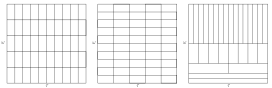
\includegraphics[width=\linewidth]{./figures/stft_cwt_grid/stft_cwt_grid.pdf}
        \caption{
        \textit{Left/middle:} The figures illustrates the tradeoff in resolution for time and frequency for the short-time Fourier transform from equation \eqref{eq:stft}, increasing the resolution in time decreases the resolution in frequency and vice versa.
\textit{Right:} Illustrate the corresponding resolution for the continuous wavelet transform from equation \eqref{eq:cwt}.
}
        \label{fig:grid}
\end{figure}
This is very intuitive as frequency has to be measured over a certain time period.
Decreasing the width of the window function makes detecting smaller frequencies harder, and vice versa.
Thus we need to know the approximate frequency scales in the data before performing the STFT, or we can try several window widths.
In the case where frequencies exists in the data on several different scales, the STFT in equation \eqref{eq:stft} becomes unsuitable.



\subsection{Wavelet Transform}
The wavelet transform works in a very similar way as the STFT, but circumvents the problem of choosing a fixed width of the window by introducing scaling.
Let $\psi(t)$ be a window function (possibly complex valued) which we will call the mother wavelet.
One way of scaling the mother wavelet by a factor $s$ is
\begin{equation*}
        \psi_s(t) = \frac{1}{s^{1/2}} \psi \left(\frac{t}{s}\right).
\end{equation*}
If we also allow a time shift around $\tau$ we arrive at the wavelets
\begin{equation*}
        \psi_{s,\tau}(t) = \frac{1}{s^{1/2}} \left( \frac{t - \tau}{s} \right).
\end{equation*}
This culminates in the definition of the continuous wavelet transform (CWT) of a function $f$ \cite{kaiser}
\begin{equation}\label{eq:cwt}
        \tilde{f}(s, \tau)\int_{-\infty}^{\infty}\psi_{s,\tau}^*(t)f(t) dt,
\end{equation}
where $\psi_{s,\tau}^*$ is the complex conjugate of the function $\psi_{s, \tau}$.

Again considering the discrete sample $y_1, y_2, \hdots, y_n$ with $\delta t = y_{t+1} - y_t, \ t = 1, \hdots, n$, its continuous wavelet transform is given by \cite{torrence}
\begin{equation}\label{eq:cwt_d}
        \tilde{f}_n(s, \tau) = \sum_{t = 1}^{n} y_t \psi^* \left( \frac{\delta t}{s}(t- \tau) \right),
\end{equation}
where $\tau$ now is a time index $\tau \in \{ 1, 2, \hdots, n \}$.
It is computationally efficient \cite{torrence} to represent the CWT as the inverse Fourier transform
\begin{align*}
        &\tilde{f}_n(s, \tau) \sum_{t = 1}^{n}\hat{y}_k \hat{\psi}^*(s\omega_k)e^{i \omega_k n\delta t}, \\
        & \hat{y}_k = \frac{1}{n}\sum_{t = 1}^{n}y_t e^{-\frac{i2\pi kt}{n}},\\
        &\omega_k = 
                \begin{cases}
                      \frac{2\pi k}{n \delta t},   &  k \leq \frac{n}{2} \\
                      -\frac{2\pi k}{n \delta t},   &  k > \frac{n}{2} \\
                \end{cases}.
\end{align*}
As always we are interested in the power spectrum, which for the CWT is defined as $|\tilde{f}_n(s,\tau)|^w$.

There exists many choices for the mother wavelet, and certain important criteria it must satisfy \cite{kaiser}.
One popular wavelet is the Morlet wavelet defined as
\begin{equation}\label{eq:morlet}
        \psi_0(\eta) = \pi^{-1/4} e^{i\omega_0 \eta}e^{-\eta^2 / 2},
\end{equation}
where $\omega_0$ is a parameter chosen to fit the criteria.


















\section{Piecewise polynomials}
Suppose we have an interval $[a,b]$ divided into $M$ contiguous subintervals.
The connecting edges of the subintervals $a = \xi_0, \xi_1, \hdots, \xi_{M - 1}, \xi_{M} = b$ are called knots.
On each of the intervals $[\xi_i, \xi_{i+1}], i = 0, \hdots, M-1$ we define a polynomial $p_i (t)$.
The function
\begin{equation*}
        f(t) = 
                \begin{cases}
                        p_0(t), &  t \in [\xi_0, \xi_{1}) \\
                        p_1(t), & t \in [\xi_1, \xi_2)  \\
                        & \vdots \\
                        p_{M-1}(t), & t \in [\xi_{M-1}, \xi_{M}]  \\
                \end{cases}
\end{equation*}
is called a \textit{piecewise polynomial}.


\subsection{Splines}
In the definition of piecewise polynomials no restrictions are made on the polynomials, they are allowed to take any form.
As in \cite{quarteroni} we define a \textit{spline} $s_k(t)$ of order $k$ on the interval $[a,b]$ as a piecewise polynomial where
\begin{align*}
        &s_k(t) \in \mathcal{P}^k , \quad t \in [\xi_i, \xi_{i+1}],\quad i = 0, 1, \hdots, M-1 \\
        &s_k(t) \in \mathcal{C}^{k - 1}[a, b].
\end{align*}
I.e., the spline consists of piecewise polynomials of order $k$ and has continuous derivatives up to order $k - 1$.
A common choice is letting $k = 3$, providing continuous second derivatives over the interval.
This is called \textit{cubic} splines, and are often considered sufficiently smooth for function approximations.
It is also common to add curvature constraints at the endpoints, $s_3''(a) = s_3''(b)$, arriving at the \textit{natural} cubic splines.

\subsection{Regression splines}
Suppose now we have data points $y_{t_1}, y_{t_2}, \hdots, y_{t_n}$ on $[a = t_1, b = t_n]$. 
A spline of order $k$ with chosen knots at $a = t_1 = \xi_0, \xi_1, \hdots, \xi_{M} = t_n = b$ can be parameterized as 
\begin{equation}\label{eq:lsq_spline}
        s_k(t) = \sum_{i = 1}^{M + k} \beta_i h_i(t),
\end{equation}
where the functions $h_i$ are the truncated-power basis set
\begin{align*}
        h_j(t) &= t^{j - 1}, \ j = 1, \hdots, k+1, \\
        h_{k+1+l}(t) &= (t - \xi_l)_+^k, \ l = 1, \hdots, M-1,
\end{align*}
with $(t)_+ = \max_{} \{ t, 0 \}$ \cite{hastie}.
The parameters $\beta_i$ can be found using least squares.
An example of cubic spline regression are shown in figure \ref{fig:cubic_splines}.

\begin{figure}[tb ]
        \centering
        \includegraphics[width=\linewidth]{./code/figures/cubic_splines.pdf}
        \caption{Two cubic splines fitted using least square regression on the time series from figure \ref{fig:time_series_example}.
        Observe that the red spline with 50 knots (including endpoints) fits the data closer than the green spline with 10 knots.}
        \label{fig:cubic_splines}
\end{figure}




\section{Dimensionality reduction}
\subsection{Principal Component Analysis}
\subsection{t-Stochastic Neighbor Embedding}
\section{Watershed segmentation}




\chapter{Methodology}
The starting point of the analysis is a set $\textbf{Y} =  \{ Y_d : d = 1, 2, \hdots, D \}$, where each set $Y_d$ is again a set of independent time series, $Y_d = \{ y_1^d(t), y_2^d(t), \hdots, y_n^d(t): t \in \{t_1, t_2, \hdots, t_{m_d} \} \}$.
Each $Y_d$ represents an animal for which $n$ time series are collected tracking parts of its movements.
Recording frequency is the same across animals.
The goal of the analysis is to cluster these time points into distinct distinguishable actions.

\textcolor{red}{Some summarization: "This is achieved by..."}

\section{Feature extraction}
The first step is to analyse each time series separately, modifying them and thus creating $D \times n$ features which we will extract the behavioral information from.
Let $y_t = \{ y_1, y_2, \hdots, y_m \} = y_i^d(t)$ for some $d \in \{ 1, 2, \hdots, D \}$ and $i \in \{ 1, 2, \hdots, n \}$ be one such series.

\textcolor{red}{I don't see the point in centering the data around the mean before the detrending.}

We detrend the data as $y_t = s_3(t) + x_t$, $s_3(t)$ being the non-linear trend and $x_t$ the detrended time series.
The cubic spline $s_3(t)$ is found using least square regression as in equation \eqref{eq:lsq_spline} with equally spaced internal knots $\xi_1, \xi_2, \hdots, \xi_M$.
We choose the knots to have a fixed frequency, i.e., we choose $\Delta \xi= \xi_{i+1} - \xi_i, i = 2, \hdots, M$.
Figure \ref{fig:detrending_bc} shows an example of a detrended time series using cubic splines with interior knots every 240th time point.


\begin{figure}[tb ]
        \centering
        \includegraphics[width=\linewidth]{./code/figures/detrending_bc.pdf}
        \caption{Detrended time series using cubic spline regression.
        The top figure shows the original time series in black with the fitted trend in red.
The bottom figure shows the detrended time series.}
        \label{fig:detrending_bc}
\end{figure}

\section{Manifold embedding}








\newpage
\printbibliography
\end{document}



